% This is "sig-alternate.tex" V2.0 May 2012
% This file should be compiled with V2.5 of "sig-alternate.cls" May 2012
%
% This example file demonstrates the use of the 'sig-alternate.cls'
% V2.5 LaTeX2e document class file. It is for those submitting
% articles to ACM Conference Proceedings WHO DO NOT WISH TO
% STRICTLY ADHERE TO THE SIGS (PUBS-BOARD-ENDORSED) STYLE.
% The 'sig-alternate.cls' file will produce a similar-looking,
% albeit, 'tighter' paper resulting in, invariably, fewer pages.
%
% ----------------------------------------------------------------------------------------------------------------
% This .tex file (and associated .cls V2.5) produces:
%       1) The Permission Statement
%       2) The Conference (location) Info information
%       3) The Copyright Line with ACM data
%       4) NO page numbers
%
% as against the acm_proc_article-sp.cls file which
% DOES NOT produce 1) thru' 3) above.
%
% Using 'sig-alternate.cls' you have control, however, from within
% the source .tex file, over both the CopyrightYear
% (defaulted to 200X) and the ACM Copyright Data
% (defaulted to X-XXXXX-XX-X/XX/XX).
% e.g.
% \CopyrightYear{2007} will cause 2007 to appear in the copyright line.
% \crdata{0-12345-67-8/90/12} will cause 0-12345-67-8/90/12 to appear in the copyright line.
%
% ---------------------------------------------------------------------------------------------------------------
% This .tex source is an example which *does* use
% the .bib file (from which the .bbl file % is produced).
% REMEMBER HOWEVER: After having produced the .bbl file,
% and prior to final submission, you *NEED* to 'insert'
% your .bbl file into your source .tex file so as to provide
% ONE 'self-contained' source file.
%
% ================= IF YOU HAVE QUESTIONS =======================
% Questions regarding the SIGS styles, SIGS policies and
% procedures, Conferences etc. should be sent to
% Adrienne Griscti (griscti@acm.org)
%
% Technical questions _only_ to
% Gerald Murray (murray@hq.acm.org)
% ===============================================================
%
% For tracking purposes - this is V2.0 - May 2012

\documentclass{sig-alternate}
\usepackage{subfigure}
\usepackage{color}
\usepackage{algorithm}
\usepackage{algorithmic}
\usepackage{caption2}
\usepackage{multirow} %multirow for format of table
\usepackage{amsmath}
\usepackage{xcolor}
\renewcommand{\algorithmicrequire}{\textbf{Input:}}
\renewcommand{\algorithmicensure}{\textbf{Output:}}
\def\sharedaffiliation{
\end{tabular}
\begin{tabular}{c}}

\begin{document}
%
% --- Author Metadata here ---
\conferenceinfo{ICIMCS'14,} {July 10--12, 2014, Xiamen, Fujian, China.}
\CopyrightYear{2014}
\crdata{978-1-4503-2810-4/14/07}
\clubpenalty=15000
\widowpenalty = 15000
% --- End of Author Metadata ---

\title{Learning Hash Functions Using Sparse Reconstruction}
%\subtitle{[Extended Abstract]
%\titlenote{A full version of this paper is available as
%\textit{Author's Guide to Preparing ACM SIG Proceedings Using
%\LaTeX$2_\epsilon$\ and BibTeX} at
%\texttt{www.acm.org/eaddress.htm}}}
%
% You need the command \numberofauthors to handle the 'placement
% and alignment' of the authors beneath the title.
%
% For aesthetic reasons, we recommend 'three authors at a time'
% i.e. three 'name/affiliation blocks' be placed beneath the title.
%
% NOTE: You are NOT restricted in how many 'rows' of
% "name/affiliations" may appear. We just ask that you restrict
% the number of 'columns' to three.
%
% Because of the available 'opening page real-estate'
% we ask you to refrain from putting more than six authors
% (two rows with three columns) beneath the article title.
% More than six makes the first-page appear very cluttered indeed.
%
% Use the \alignauthor commands to handle the names
% and affiliations for an 'aesthetic maximum' of six authors.
% Add names, affiliations, addresses for
% the seventh etc. author(s) as the argument for the
% \additionalauthors command.
% These 'additional authors' will be output/set for you
% without further effort on your part as the last section in
% the body of your article BEFORE References or any Appendices.

\numberofauthors{3}
\author{
% You can go ahead and credit any number of authors here,
% e.g. one 'row of three' or two rows (consisting of one row of three
% and a second row of one, two or three).
%
% The command \alignauthor (no curly braces needed) should
% precede each author name, affiliation/snail-mail address and
% e-mail address. Additionally, tag each line of
% affiliation/address with \affaddr, and tag the
% e-mail address with \email.
%
% 1st. author
Yong Yuan, Xiaoqiang Lu, Xuelong Li
%\alignauthor XXXXX\\
% 2nd. author
%\alignauthor XXXXX\\
%% 3rd. author
%\alignauthor XXXXX\\
%\and  % use '\and' if you need 'another row' of author names
\sharedaffiliation
       \affaddr{Center for OPTical IMagery Analysis and Learning (OPTIMAL),}\\
       \affaddr{State Key Laboratory of Transient Optics and Photonics, Xi'an Institute of Optics and Precision Mechanics,}\\
       \affaddr{Chinese Academy of Sciences, Xi'an 710119, Shaanxi, P. R. China.}\\
       \email{yuanyong@opt.cn}, \email{\{luxiaoqiang, xuelong\_li\}}{@opt.ac.cn}\\
}
% There's nothing stopping you putting the seventh, eighth, etc.
% author on the opening page (as the 'third row') but we ask,
% for aesthetic reasons that you place these 'additional authors'
% in the \additional authors block, viz.
%\additionalauthors{Additional authors: John Smith (The Th{\o}rv{\"a}ld Group,
%email: {\texttt{jsmith@affiliation.org}}) and Julius P.~Kumquat
%(The Kumquat Consortium, email: {\texttt{jpkumquat@consortium.net}}).}
%\date{30 July 1999}
% Just remember to make sure that the TOTAL number of authors
% is the number that will appear on the first page PLUS the
% number that will appear in the \additionalauthors section.

\maketitle
\begin{abstract}
\emph{Approximate nearest neighbor} (ANN) search is becoming an increasingly important technique in large-scale problems. Recently many approaches have been developed due to fast query and low storage cost. Although most of them have realized the importance of the data structure, they neglected the sparse relationship of the data. To  build a balance between the adjusted covariance matrix and the minimum reconstruction error of data points, this paper proposes a novel method based on sparse reconstruction to learn more compact binary codes under $l_{2,1}$-norm constraint. Experiments demonstrate that the proposed method, named as sparse reconstruction hashing, outperforms several other state-of-the-art methods when tested on a few benchmark datasets.
\end{abstract}

% A category with the (minimum) three required fields
\category{H.3.3}{Information Search and Retrieval}{Retrieval models}
%A category including the fourth, optional field follows...
%\category{D.2.8}{Software Engineering}{Metrics}[complexity measures, performance measures]

\terms{Algorithms, Experimentation, Performance}

\keywords{Image search, ANN, hashing, sparse reconstruction}

\section{Introduction}

\emph{Nearest neighbor} (NN) search has been widely applied to large-scale vision problems including image retrieval, object recognition and many other computer vision problems. Recently, with the explosive growth of data, many research efforts have been devoted to investigating the alternative solution-ANN search, which allows fast search in large database. To address this problem, most of tree-based methods have been proposed. However, for high-dimensional data, the performance of tree-based methods suffer significantly with their performance drastically degrading to exhaustive linear search. Besides, since the data structure based on tree is bigger than the original data itself, it also suffers from memory constraints.

To overcome these issues, many researchers have proposed to use hashing technique for ANN search. There is a general consensus among these researchers that semantically similar data points should be mapped to the same or close hash buckets in ANN search. One of the greatest advantage of hashing-based techniques is that the query time is constant or sub-linear. Moreover, the storage reduces substantially as they learn compact codes representation for the data while preserving the similarity structure of the original feature space. Hence, hashing-based methods can achieve fast query time with low storage requirement, which provide a popular candidate for efficient ANN search in large-scale datasets.

Currently, a lot of hashing-based methods have been proposed to design effective compact hash functions. According to whether they make use of dataset to learn the hash functions, hashing-based methods can be roughly divided into two categories, i.e. data-independent hashing methods and data-dependent hashing methods.

Data-independent hashing methods usually construct a set of hash functions using randomization without training stage. The representative data-independent methods include Local Sensitive Hashing (LSH) \cite{DBLP:vldbGionisIM99-01}, its extension and Shift-Invariant Kernel-based Hashing (SIKH) \cite{DBLP:nipsRaginskyL09-02}. Due to the data-blindness, data-independent hashing methods usually need a large number of bits and neglect data internal structure. Besides, longer codes decrease greatly the collision probability between close data samples in the original space. Hence, multiple hash tables are introduced to enlarge the probability to achieve reasonable recall, but this results in increase of query time and big storage requirement.

In general, data-dependent hashing methods are shown to be superior to data-independent hashing methods. Unlike data-independent hashing methods, data-dependent hashing methods can make use of learning techniques to construct a set of hash functions. According to whether they make use of the label information or not, the data-dependent hashing methods can be summarized into three categories, namely supervised, semi-supervised \cite{DBLP:WangKC10-16} and unsupervised hashing methods.

Supervised hashing methods try to take advantage of labeled training samples to improve hashing performance such as \iffalse Boosted Similarity Sensitive Coding (BSSC) \cite{phdthesis:shakhnarovich2005-04},\fi Semantic Hashing \cite{DBLP:SalakhutdinovH09-05}, Binary Reconstructive Embedding (BRE) \cite{DBLP:nipsKulisD09-06}, and Kernel-based Supervised Hashing (KSH) \cite{DBLP:cvprLiuWJJC12-07}. However, the main problem with the existing supervised hashing techniques is that they need many labeled samples, which is a tough task to label when the database is large.

 To handle the aforementioned problem, unsupervised hashing methods, including Kernelized Locality-Sensitive Hashing (KLSH) \cite{DBLP:conf/iccvKulisG09-08}, Spectral Hashing (SH) \cite{DBLP:WeissTF08-09}, Multidimensional Spectral Hashing (MDSH) \cite{DBLP:eccvWeissFT12-10}, PCA-ITQ \cite{DBLP:cvprGongL11-11}, and K-Means Hashing (KMH) \cite{DBLP:HeWS13-03}, can achieve binary codes from given data samples by unsupervised learning. Since unsupervised methods don't need labeled data, they can be widely applied to different data domains.

In this paper, we focus on unsupervised method and propose a novel method using sparse reconstruction to learn hash functions. First, $l_{21}$-norm is introduced into \emph{sparsity preserving projections} (SPP) framework to preserve potential discrimination information of hash functions. Second, we construct an objective function to build a balance between the adjusted covariance matrix and the minimum reconstruction error of data points. The main contributions of this paper are briefly outlined as follows:
\begin{itemize}
\setlength\baselineskip{9.4pt}
  \item It has been pointed out that SPP contains natural discriminating information. To make full use of the advantage, a novel sparse reconstruction method is proposed to learn hash functions. Furthermore, the proposed method uses a $l_{21}$-norm instead of $l_1$-norm to capture some intrinsic geometric information of hash functions.
  \item The proposed method takes both information entropy maximum and data structure into consideration simultaneously. To the best of our knowledge, most of existing hashing methods treat them  as two independent phases, but actually they may be inter-related. The proposed method considers them simultaneously and we present an efficient algorithm to solve the formulation.
\end{itemize}
The rest of the paper is organized as follows: Section 2 reviews related work. Section 3 presents the details of our method including optimization method. Section 4 gives comparison results to evaluate the effectiveness of the proposed method. Section 5 concludes the paper.

\section{Related Work}

Since some annotations will be used later, we first introduce them for convenience. Suppose the dataset $X \in R^{d \times N}$ consists of N data points \{$x_i$\}$_{i=1}^N$, $x_i \in R^d$.  The purpose of hashing-based method tries to learn a set of hash functions $h_k(x)\in H$ $(k=1, 2, \cdots, K)$ to map each data point $x_i$ to a $K$-bit low-dimensional hash code $H(x_i)=[h_1(x_i), h_2(x_i), \cdots, h_K(x_i)]$, where $h_k(x_i)$ belongs to \{-1,1\}. Assuming the data points are zero-centered, for each bit $k=1, \cdots, K$, the binary encoding function is defined as $h_k(x_i) = sgn(w_k^Tx_i)$, where $w_k$ is a column vector of hyperplane coefficient. The function $sign(v)$ is defined as 1 if input variable $v>0$ and -1 otherwise.

Following the formulation of \cite{DBLP:WeissTF08-09}, in order to generate an efficient code, each bit requires a 50\% chance of being one or zero. According to information theory's maximum entropy rule, the variance of hash functions are required to be maximized and the following objective function can be obtained:
\begin{equation}\label{eqj11}
    \begin{split}
J_1(W) &=\sum_{k=1}^{K}var(h_k(x))=\sum_{k=1}^{K}var(sgn(w_k^Tx)).\\
    \end{split}
\end{equation}
As shown in \cite{DBLP:cvprGongL11-11}, solving the objective function in Eq.\ref{eqj11} is intractable since the requirement of exact balancedness makes the above objective function intractable. By relaxing the signed magnitude as shown in \cite{DBLP:WangKC10-16}, the objective function \eqref{eqj11} can be transformed as follows:
\begin{equation}\label{eqj12}
    \begin{split}
\tilde{J_1}(W) &=\sum_{k=1}^{K}E(||w_k^Tx||_2^2)=\frac{1}{n}\sum_{k=1}^{K}w_k^TXX^Tw_k\\
 &= \frac{1}{n}tr(W^TXX^TW).\\
    \end{split}
\end{equation}

For a pair of points $x_i$ and $x_j$, if $x_i$ and $x_j$ are similar to each other, it's important for hash functions to encourage them to be encoded into similar binary codes since the corresponding weight $t_{i, j}$ between them is large. Hence  it's reasonable to maximize the following objective function according to \cite{DBLP:iccvXuWLZLY11-12}:
\begin{equation}\label{eqj21}
    \begin{split}
\tilde{J_2}(W)=\sum_{i,j=1}^{N}t_{ij}<H(x_i), H(x_j)>,\\
    \end{split}
\end{equation}
where the weight element $t_{i, j}$ ($T$ is the corresponding matrix) is denoted the same as $s_{i, j}$ in \cite{DBLP:iccvXuWLZLY11-12}. By relaxing the $sgn(w^Tx)$ to the signed magnitude, the objective function in Eq.\ref{eqj21} can be rewritten as:
\begin{equation}\label{eqj22}
    \begin{split}
\tilde{J_2}(W) &=\sum_{i,j=1}^{N}t_{ij}H(x_i)^TH(x_j)=\sum_{i,j=1}^{N}t_{ij}(W^Tx_i)^TW^Tx_i\\
 &= tr(W^TXTX^TW).\\
    \end{split}
\end{equation}
By considering the regularization term in Eq.\eqref{eqj12}, Eq.\eqref{eqj22} can be transformed as follow:
\begin{equation}\label{eqj23}
    \begin{split}
\tilde{J_2}(W) &=\max_{W} tr(W^TXTX^TW+\lambda W^TXX^TW)\\
 &=\max_{W} tr(W^TMW),\\
    \end{split}
\end{equation}
where $M=XTX^T+\lambda XX^T$ is a $d \times d$ matrix, which can be referred as the adjusted covariance matrix \cite{DBLP:WangKC10-16}. $\lambda$ is the regularized parameter in Eq.\ref{eqj23}. The first term maps the similar points in the original space to the same or close buckets. The second term guarantees each bit contains maximum information.
\section{The Proposed Method}
SPP is a popular reconstruction technique, which aims to preserve the sparse reconstructive relationship of the data. The main advantage of SPP is that it contains discriminating information since sparse representation has natural discriminating power. For a given sample $x_i$, it's expected to sparsely represent each data point from the dataset $X$. The reconstruction estimation for sparse representation of $x_i$ can be obtained by minimizing the loss function under a penalized constraint:
\begin{equation}\label{eqpa1}
    \begin{split}
&\min_{s_i}||s_i||_1\\
&s.t. \ x_i=Xs_i, i=1,2,...,N\\
&1=1^Ts_i,\\
    \end{split}
\end{equation}
where $s_i \in R^N$ is a sparse coefficient vector. It's reasonable to treat $S=[s_1, s_2,\cdots,s_N]$ as the affinity weight matrix since the element $s_{ij}$ in $S$ reflects a close relation between $x_i$ and $x_j$. The $l_1$-norm $||\cdot||_1$ guarantees the sparsity of $s_{ij}$, that is, many elements in vector $s_i$ are zeros. The weight matrix $S$ not only can measure the similarity among different samples, but also may captures intrinsic structure information due to the element $s_i$ invariant to rotations and rescalings. Moreover, the nonzero entries in the sparse matrix $S$ may help to distinguish the samples from the given class even if no class-labels provided, thus the sparse reconstructive weight vector tends to contain potential discriminant information.
\begin{figure}
%\label{fignorm1}
\centering
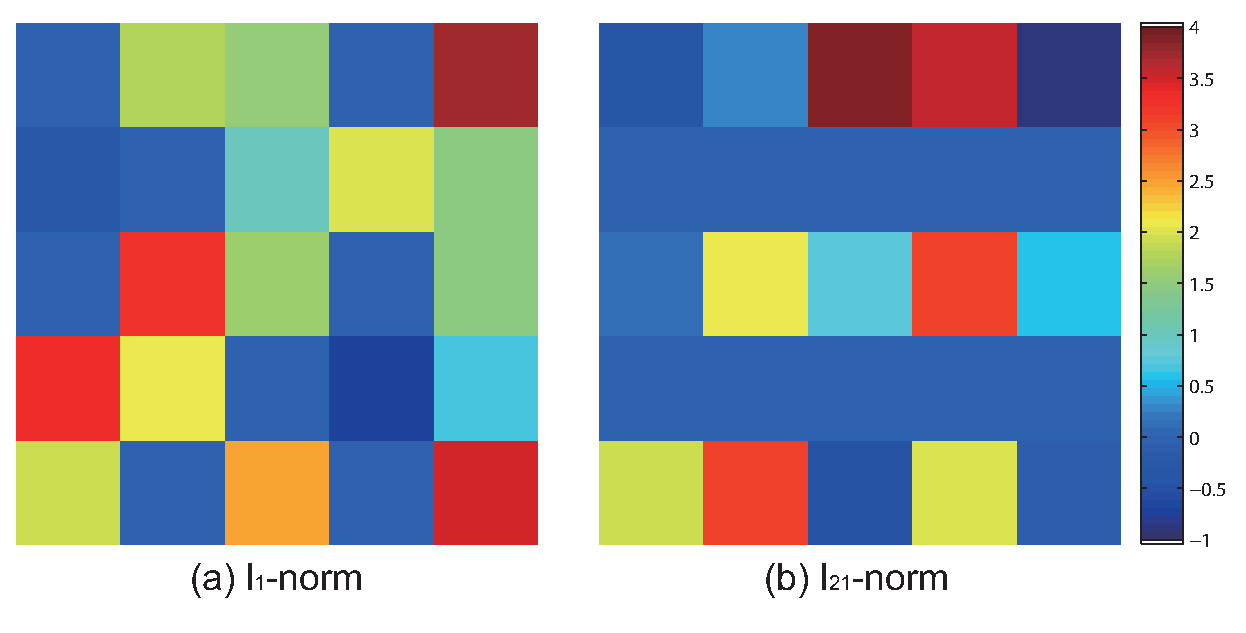
\includegraphics[width=0.45\textwidth]{images/norm.eps}
\caption{Illustration for the sparse weight matrix by (a) $l_1$-norm and (b) $l_{2,1}$-norm}\label{fignorm1}
\end{figure}
Ding and zhou (2006) first introduced the $l_{2,1}$-norm of a matrix as a rotational invariant $l_{1}$-norm, and it has attracted increasing attention. Fig. \ref{fignorm1} illustrates a matrix under $l_{1}$-norm constraint compared with $l_{2,1}$-norm. From Fig. \ref{fignorm1}, the $l_{2,1}$-norm has a structured sparsity attribute compared with $l_1$-norm. Generally, $l_{2,1}$-norm based priors offer a general way to take the structure into consideration, therefore the $l_{2,1}$-norm constraint on matrix $S$ has potential discrimination.

In this paper, by imposing the $l_{2,1}$-norm on $S$, the set of hash functions can be obtained $h_k(x)\in H(k=1,2,...,K)$ from the following objective function:
\begin{equation}
\begin{array}{l}
\mathop {\min }\limits_{{h_k},S} \sum\limits_{k = 1}^K {\sum\limits_{i = 1}^N {{{\left\| {{h_k}({x_i}) - {h_k}(X{s_i})} \right\|}^2}} }  + \alpha {\left\| S \right\|_{2,1}},\\
\end{array}
\label{eq:sparse}
\end{equation}
%\begin{equation}
%\label{eq:sparse}
%    \begin{split}
%\min_{h_k,s_i}\sum_{k=1}^{K}\sum_{i=1}^{N}||h_k(x_i)-h_k(Xs_i)||^2+\alpha||S||_{2,1}\\
%    \end{split}
%\end{equation}
where $\alpha$ is a balance parameter to adjust the importance of structure sparsity. The first term in Eq.\ref{eq:sparse} tries to reconstruct each data point to obtain the minimal loss of hash functions. The last term $l_{2,1}$-norm of matrix $S$ regularizes all the elements $\left\{s_i\right\}_{i=1}^N$ corresponding to the training dataset and is defined as $||S||_{2,1}=\sum_{i=1}^{N}||s_{i}||$. $s_{i}$ is denoted as the $ith$ column of $S$.

As mentioned in the related work, the binary encoding hash functions are defined as $h_k(x_i)=sgn(w_k^Tx_i),(k=1, 2, \cdots, K)$. It's not easy to solve the Eq.\ref{eq:sparse} due to the nondifferentiability of $sgn(\cdot)$ function. In this case, we relax $sgn(w_k^Tx_i)$ to the signed magnitude $w_k^Tx_i$, and the first term in the Eq.\ref{eq:sparse} can be transformed to the following form:
\begin{equation}\label{eq:sparsefirstterm}
    \begin{split}
& \sum_{k=1}^{K} \sum_{i=1}^{N}||h_k(x_i)-h_k(Xs_i)||^2 = \sum_{k=1}^{K} \sum_{i=1}^{N}||w_k^Tx_i-w_k^TXs_i||\\
& = \mathrm{tr}\left[W^T(XX^T-XSX^T-XS^TX^T+XSS^TX^T)W\right]\\
& = \mathrm{tr}\left(W^TXHX^TW\right),\\
    \end{split}
\end{equation}
where $V=(I-S-S^T+SS^T)$. Replacing the first term in the Eq.\ref{eq:sparse} with Eq.\ref{eq:sparsefirstterm}, then the Eq.\ref{eq:sparse} can be transformed as follows:
 \begin{equation}\label{eq:sparseobject}
    \begin{split}
    \tilde{J_3}(W,S) & =\min_{W, S} \mathrm{tr}\left(W^TXVX^TW\right)+\alpha\left \| S\right \|_{2,1}.\\
    \end{split}
\end{equation}
By constructing an auxiliary function, Eq.\ref{eq:sparseobject} can be rewritten as:
 \begin{equation}\label{eq:sparseob}
    \begin{split}
    \tilde{J_3}(W, S) & =\min_{W,S} \mathrm{tr}\left(W^TXVX^TW\right)+\alpha \mathrm{tr}\left(SUS^T\right),\\
    \end{split}
\end{equation}
where $U \in R^{N \times N}$ is a diagonal matrix and its $ith$ element is defined as:
 \begin{equation}\label{diaU}
    \begin{split}
& U_{ii}=\frac{1}{2\left \| s_{i\cdot}\right \|_2}.\\
    \end{split}
\end{equation}
To build a balance between the adjusted covariance matrix in Eq.\ref{eqj23} and the minimum reconstruction error of data points in Eq.\ref{eq:sparseob}, the final objective function is proposed by minimizing the following formulation:
 \begin{equation}\label{total}
    \begin{split}
    \tilde{J}(W, S) & =\min_{W,S} \frac{{J_3}(W,S)}{{J_2}(W)}\\
& =\min_{W,S} \frac{\mathrm{tr}\left(W^TXVX^TW\right)+\alpha\mathrm{tr}\left(SUS^T\right)}{\mathrm{tr}(W^TXTX^TW+\lambda W^TXX^TW)}.\\
    \end{split}
\end{equation}

The proposed objective function in Eq.\ref{total} can be divided into two alternating steps: fixing the sparse coefficient matrix $S$ to learn the map $W$ and learning $W$ while fixing $S$. These two steps are described in detail below.

\textbf {Fix $S$ and update $W$}. When the sparse coefficient matrix $S$ is fixed, Eq.\ref{total} can be transformed as the following objective function:
 \begin{equation}\label{fixs}
    \begin{split}
\tilde{J}(W) & = \min_{W} \frac{\mathrm{tr}\left(W^TXVX^TW\right)}{\mathrm{tr}(W^TX(T+\lambda I)X^TW)}\\
& = \min_{W} \frac{\mathrm{tr}\left(W^TXVX^TW\right)}{\mathrm{tr}(W^TXGX^TW)},\\
    \end{split}
\end{equation}
where $G=(T+\lambda I)$. The solution of Eq.\ref{fixs} can be obtained by using generalized eigenvalue decomposition problem. The optimal map matrix $W$ can be obtained by picking up the eigenvectors corresponding to the first $K$ ($K$ is the length of hash codes mentioned above) smallest eigenvalues.

\textbf {Fix $W$ and update $S$}. For a fixed $W$, Eq.\ref{total} can be transformed as follow:
 \begin{equation}\label{fixw}
    \begin{split}
    \tilde{J}(S) & =\min_{S} \mathrm{tr}\left(DVD^T\right)+\alpha\mathrm{tr}\left(SUS^T\right),\\
    \end{split}
\end{equation}
where $D=W^TX$. Taking the derivative of Eq.\ref{fixw} with respect to $S$ and setting it to zeros, we can get the sparse coefficient matrix:
 \begin{equation}\label{sparses}
    \begin{split}
S=D^TD(D^TD+\alpha U)^{-1}.\\
    \end{split}
\end{equation}
Since $\left \| s_{i\cdot}\right \|_2$ may be zero in real world application, the $ith$ element in diagonal matrix $U$ can be redefined as $U_{ii}=\frac{1}{\left \| s_{i\cdot}\right \|_2+\zeta}$ ($\zeta$ is a very small constant) in practice.

From the above discussion, the proposed method is summarized in Algorithm 1.
\begin{algorithm}[htb]
\caption{Sparse Reconstruction Hashing}
\label{alg1}
\begin{algorithmic}[1]
\REQUIRE A set of training data $X$ (zero-centered), length of hash codes $K$, the parameters $\alpha$, $\beta$, $\eta$.
\ENSURE the sparse weight matrix $S$, the map matrix $W$.
% for loop
\STATE Initialize $S_0=I_{N \times N}$, and compute the diagonal matrix $U$, the $ith$ element of $U_{ii}=\frac{1}{\left \| s_{i\cdot}\right \|_2+\zeta}$.
\REPEAT
\STATE Computer the map matrix $W$ by using generalized eigenvalue decomposition problem in Eq.\ref{fixs}.
\STATE Computer the sparse matrix $S$ by Eq.\ref{sparses}.
\STATE Update the diagonal matrix $U$.
\UNTIL{convergence}
\end{algorithmic}
\end{algorithm}
\begin{figure*}[t]
  \centering
    %\subfigure[Experimental results with different $\sigma$s]{
    %\label{figsigma}
    %\includegraphics[width= 4cm,height = 4cm]{./figure/final/8pr.eps}}
    \subfigure[\tiny{Precision-Recall curve@16 bits}]{
    \label{figlambda}
    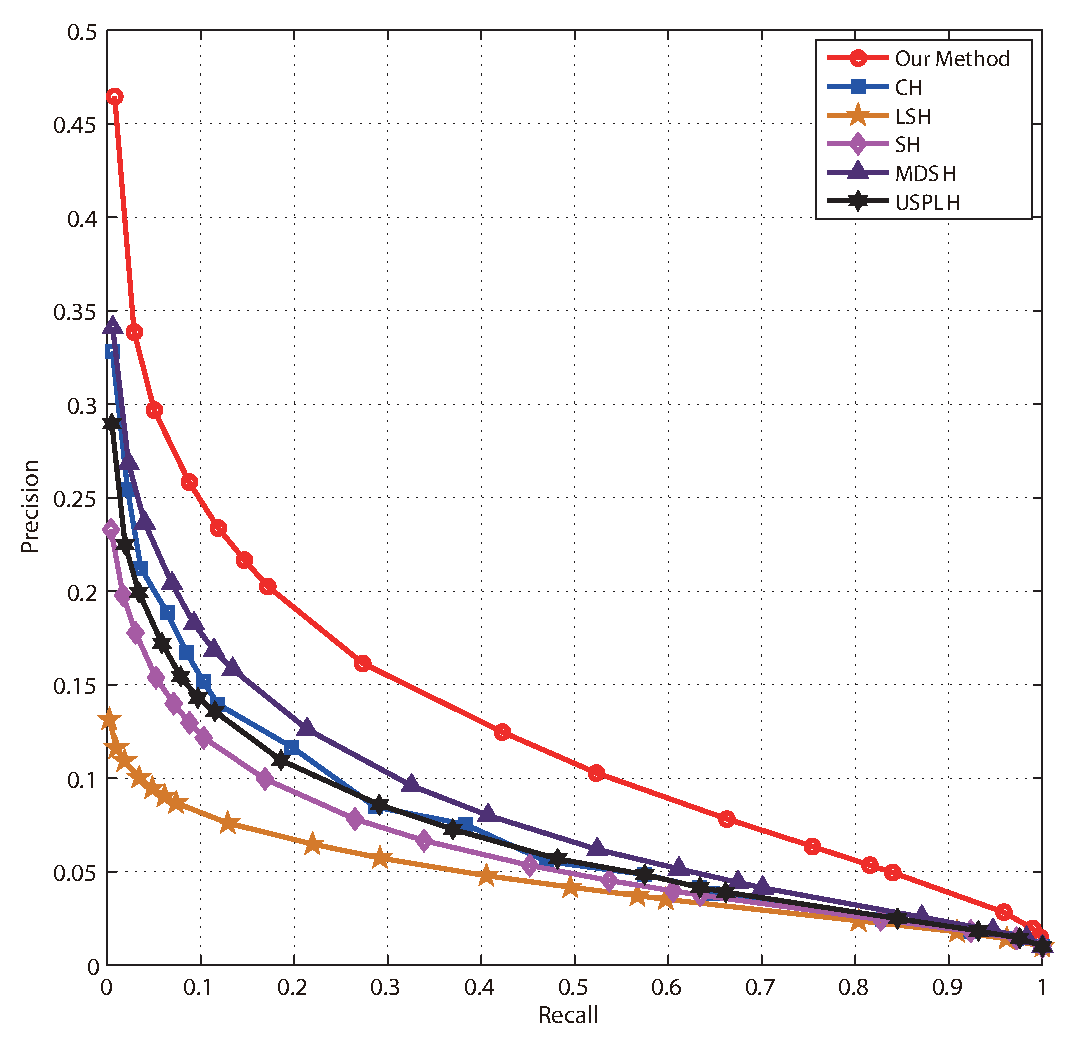
\includegraphics[width= 4.2cm,height = 4.2cm]{images/cifar10_pr_16bits.eps}}
    \subfigure[\tiny{Precision-Recall curve@24 bits}]{
    \label{figsigma}
    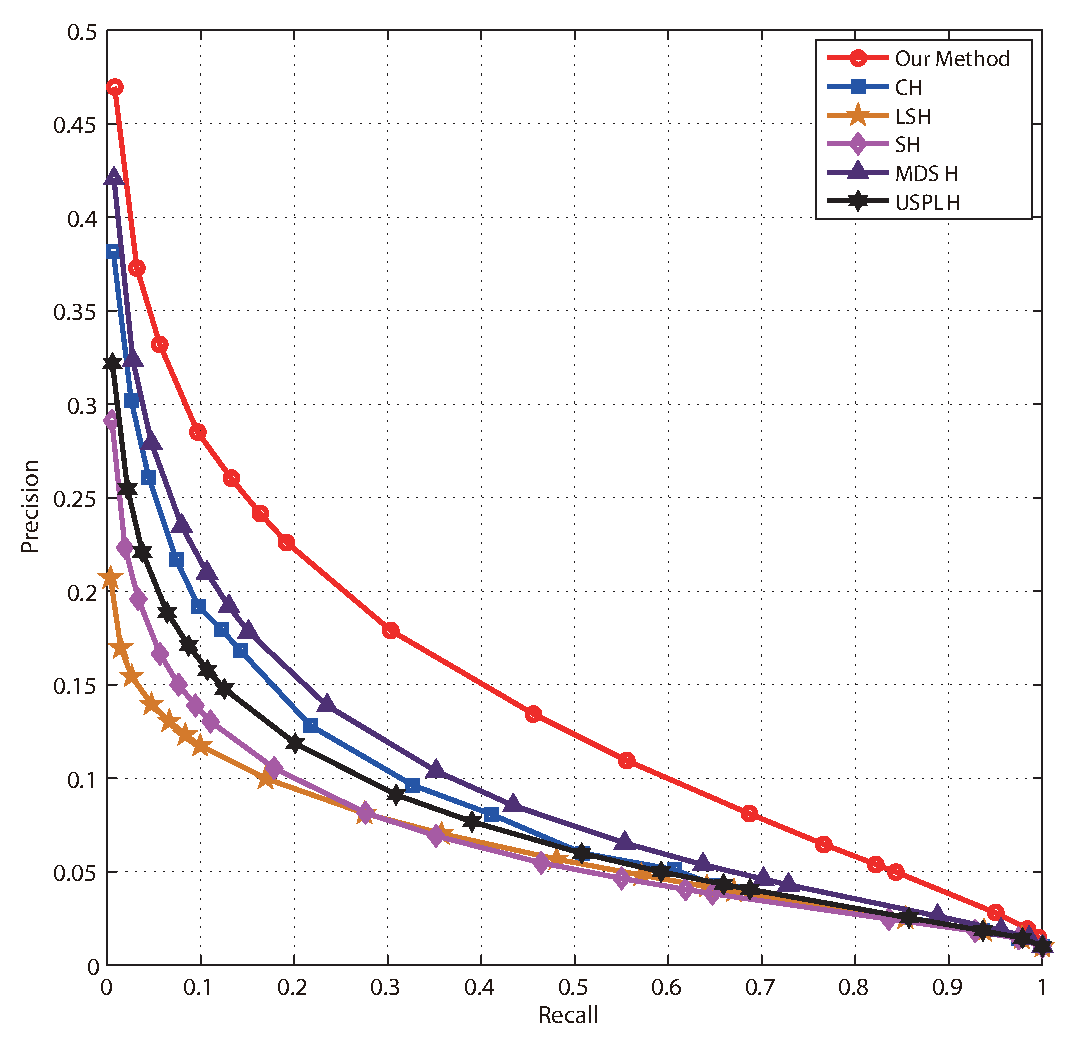
\includegraphics[width= 4.2cm,height = 4.2cm]{images/cifar10_pr_24bits.eps}}
    \subfigure[\tiny{Precision-Recall curve@32 bits}]{
    \label{figlambda}
    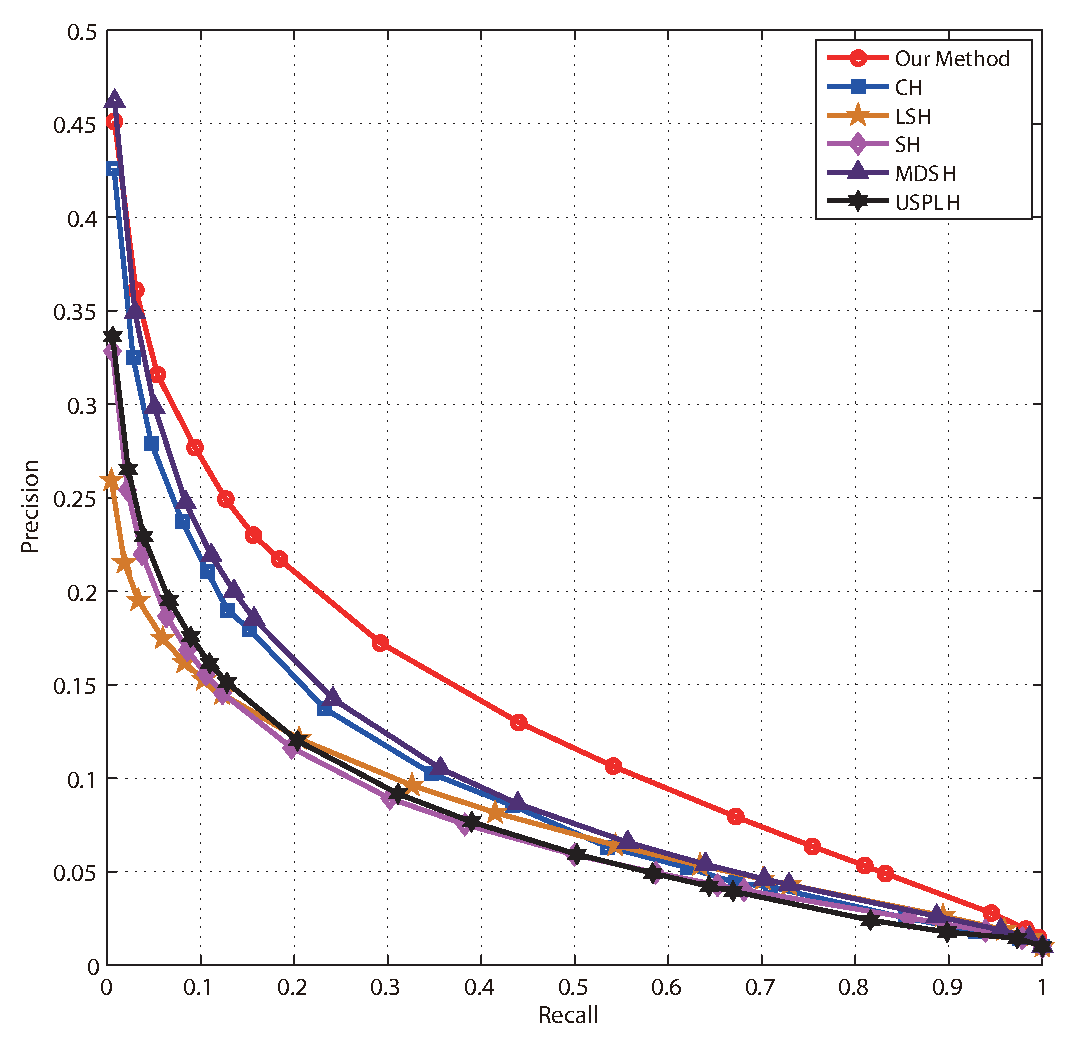
\includegraphics[width= 4.2cm,height = 4.2cm]{images/cifar10_pr_32bits.eps}}
    \subfigure[\tiny{Precision-Recall curve@48 bits}]{
    \label{figlambda}
    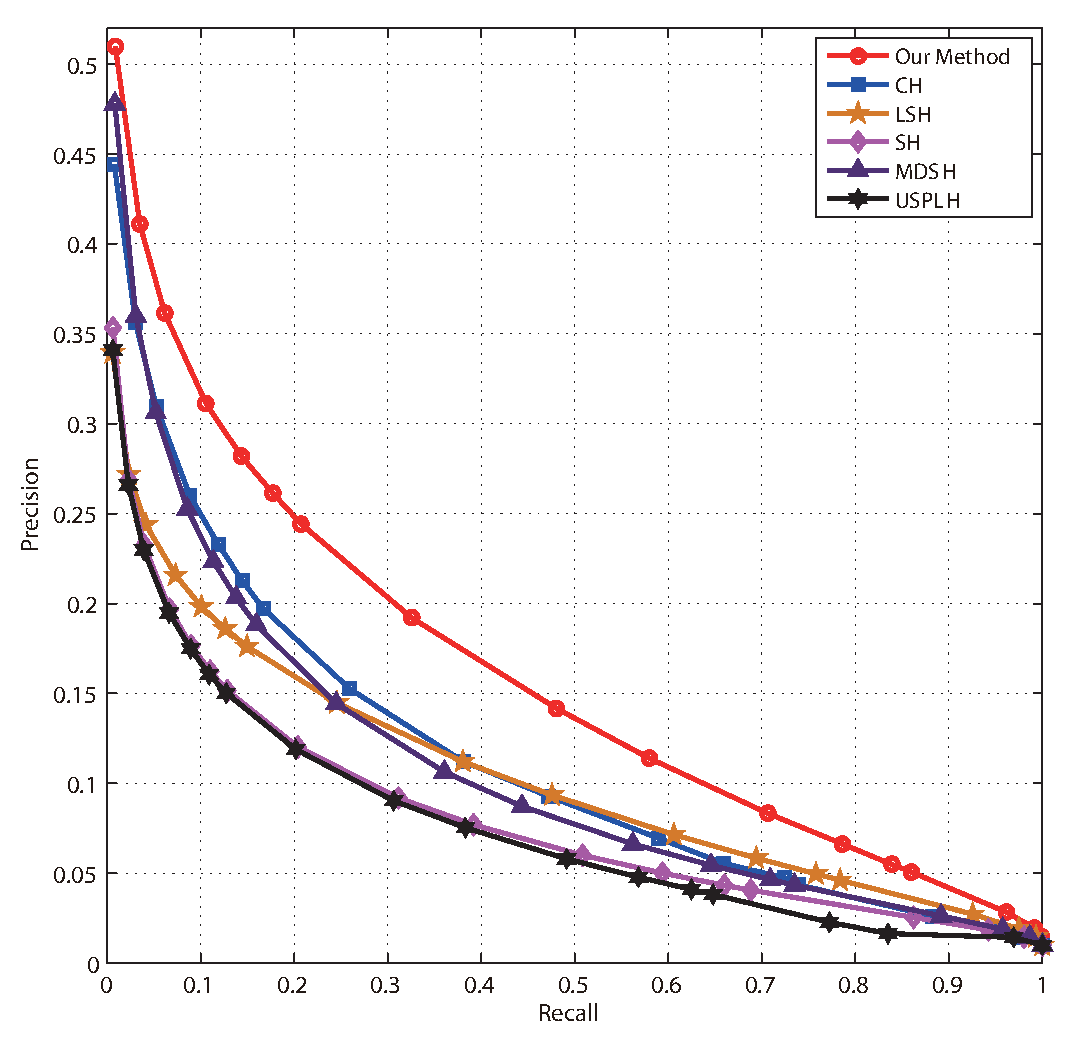
\includegraphics[width= 4.2cm,height = 4.2cm]{images/cifar10_pr_48bits.eps}}
    \subfigure[\tiny{Recall Curve @16 bits}]{
    \label{figlambda}
    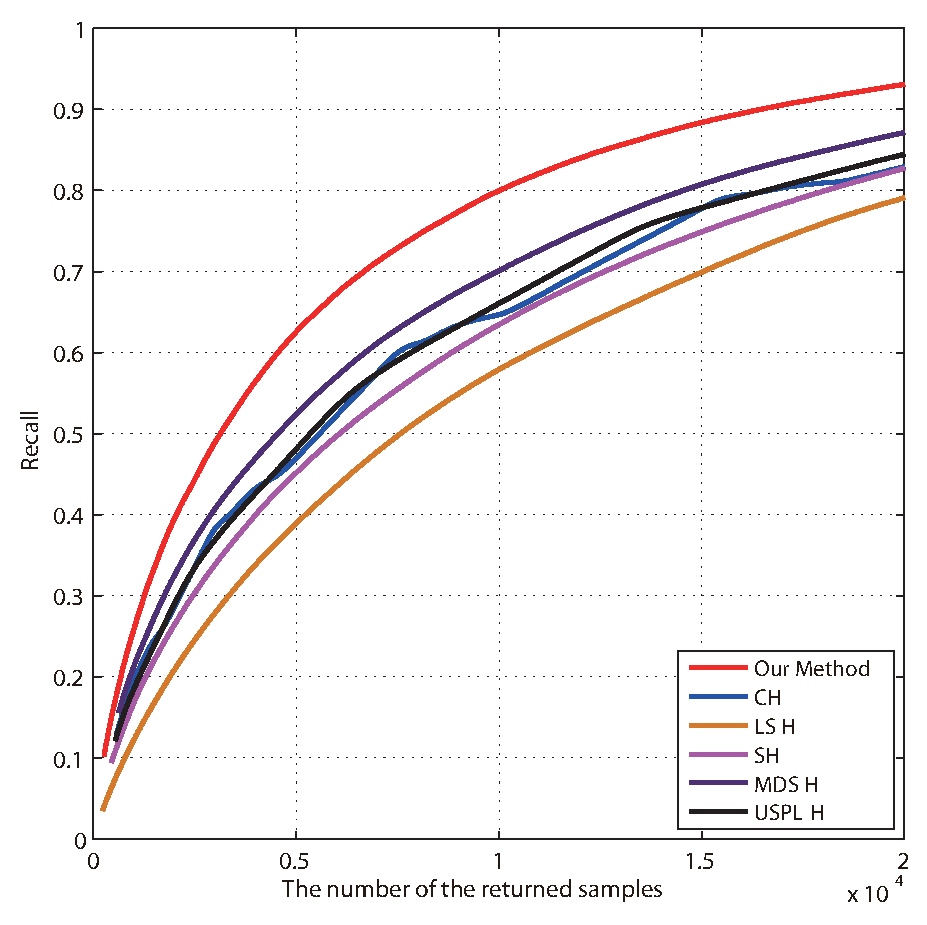
\includegraphics[width= 4.2cm,height = 4.2cm]{images/cifar10_r_16bits.eps}}
    \subfigure[\tiny{Recall Curve @24 bits}]{
    \label{figsigma}
    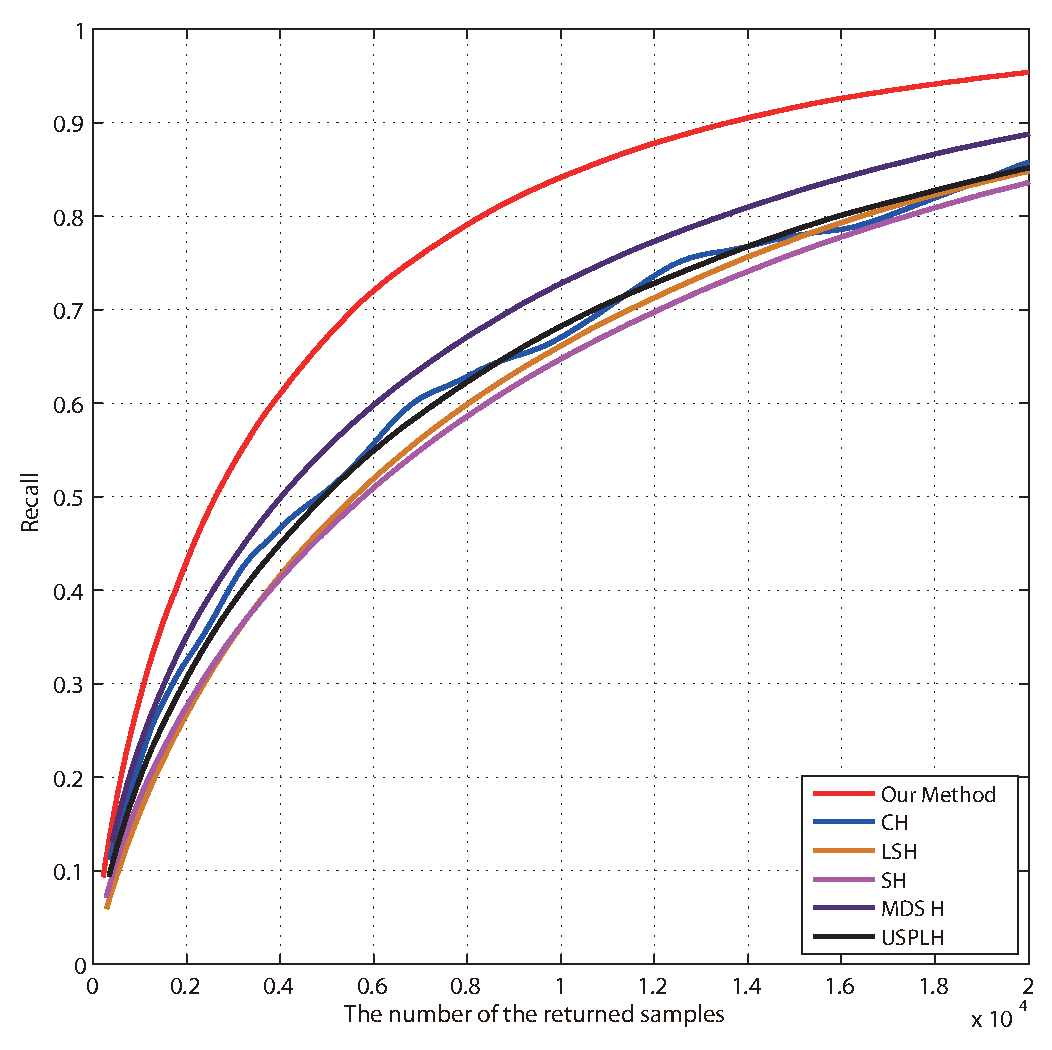
\includegraphics[width= 4.2cm,height = 4.2cm]{images/cifar10_r_24bits.eps}}
    \subfigure[\tiny{Recall Curve @32 bits}]{
    \label{figlambda}
    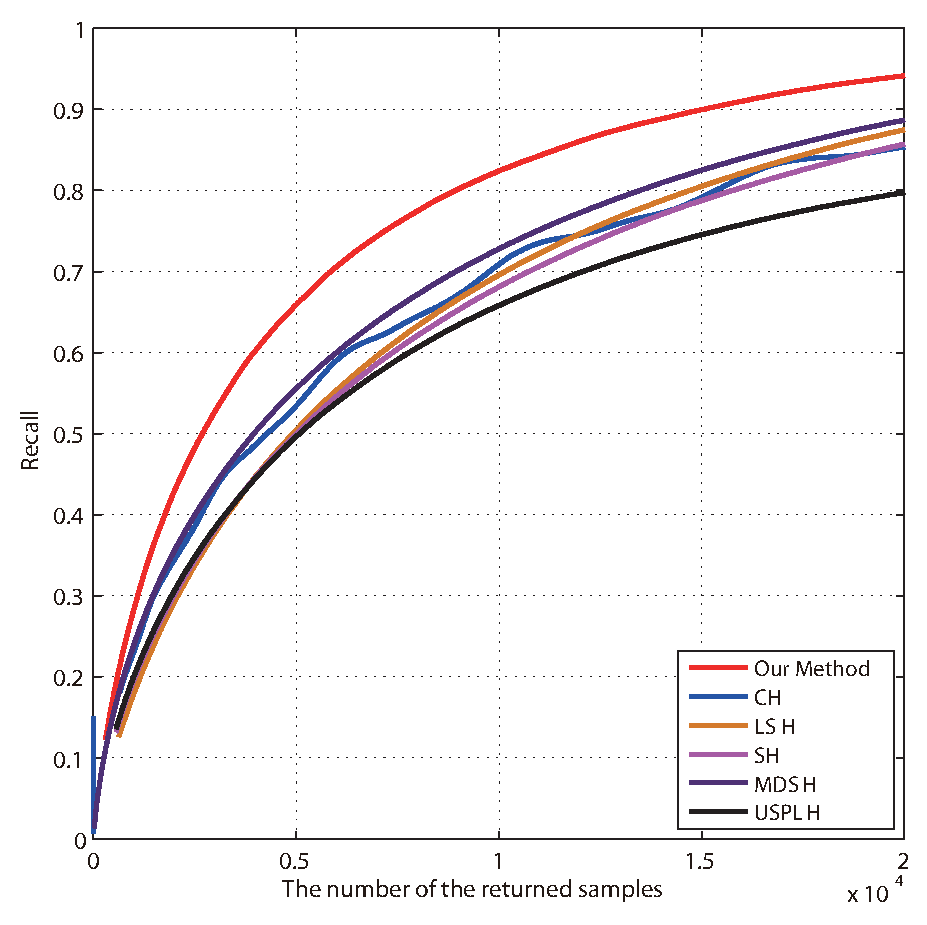
\includegraphics[width= 4.2cm,height = 4.2cm]{images/cifar10_r_32bits.eps}}
    \subfigure[\tiny{Recall Curve @48 bits}]{
    \label{figlambda}
    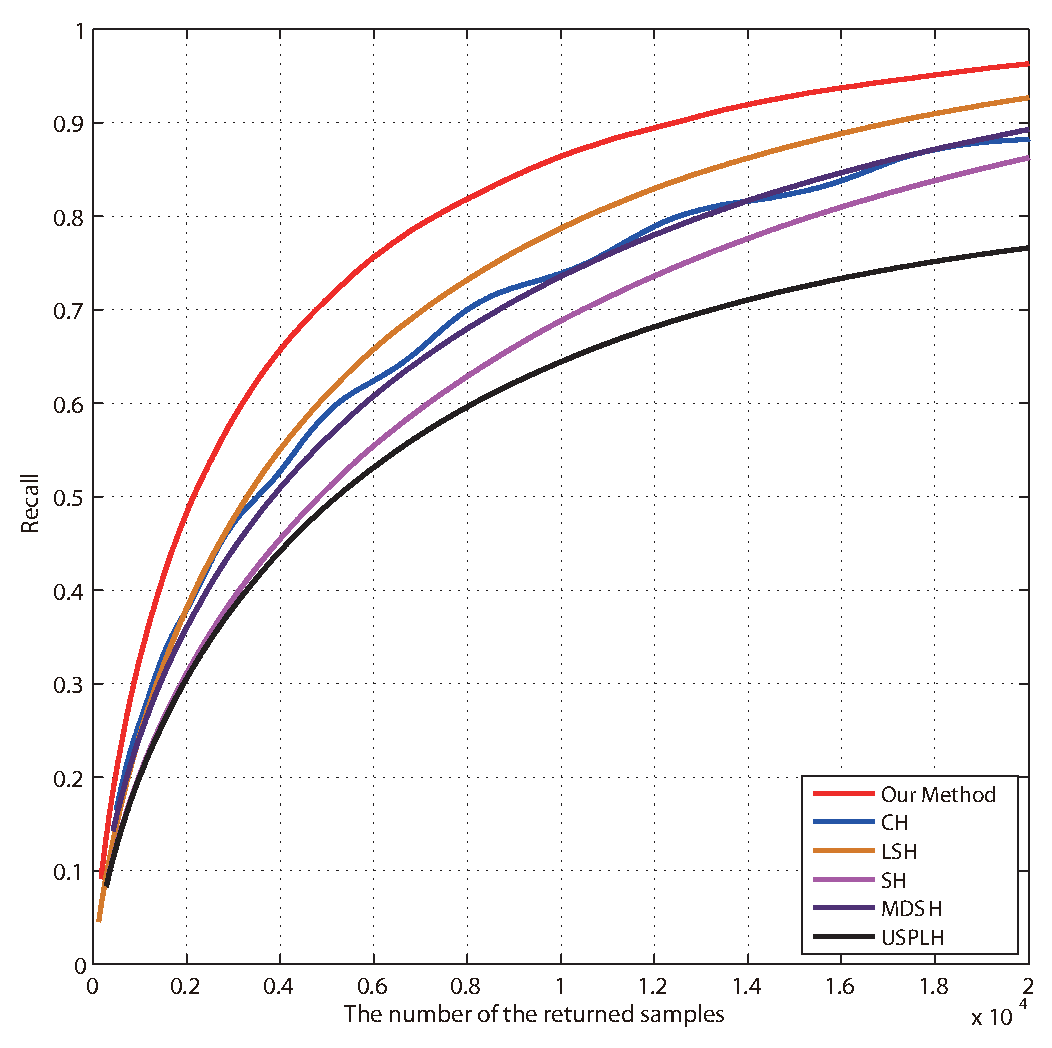
\includegraphics[width= 4.2cm,height = 4.2cm]{images/cifar10_r_48bits.eps}}
\caption{Precision-Recall curves and Recall-The number of retrieved samples curves of all approaches on cifar10 dataset.}\label{figcifar10}
\end{figure*}
\begin{figure*}[t]
  \centering
    %\subfigure[Experimental results with different $\sigma$s]{
    %\label{figsigma}
    %\includegraphics[width= 4cm,height = 4cm]{./figure/final/8pr.eps}}
    \subfigure[\tiny{Precision-Recall curve@16 bits}]{
    \label{figlambda}
    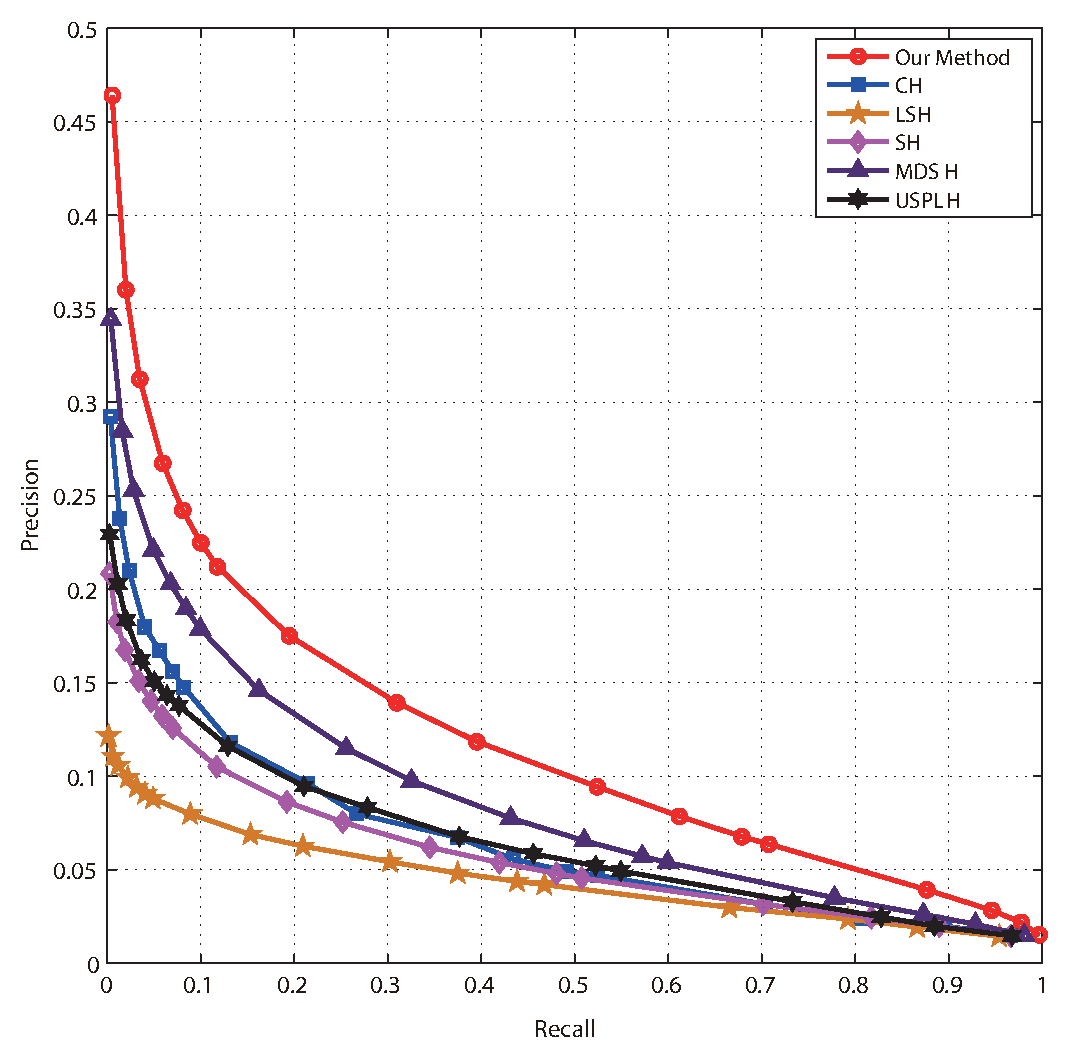
\includegraphics[width= 4.2cm,height = 4.2cm]{images/tiny100k_pr_16bits.eps}}
    \subfigure[\tiny{Precision-Recall curve@24 bits}]{
    \label{figsigma}
    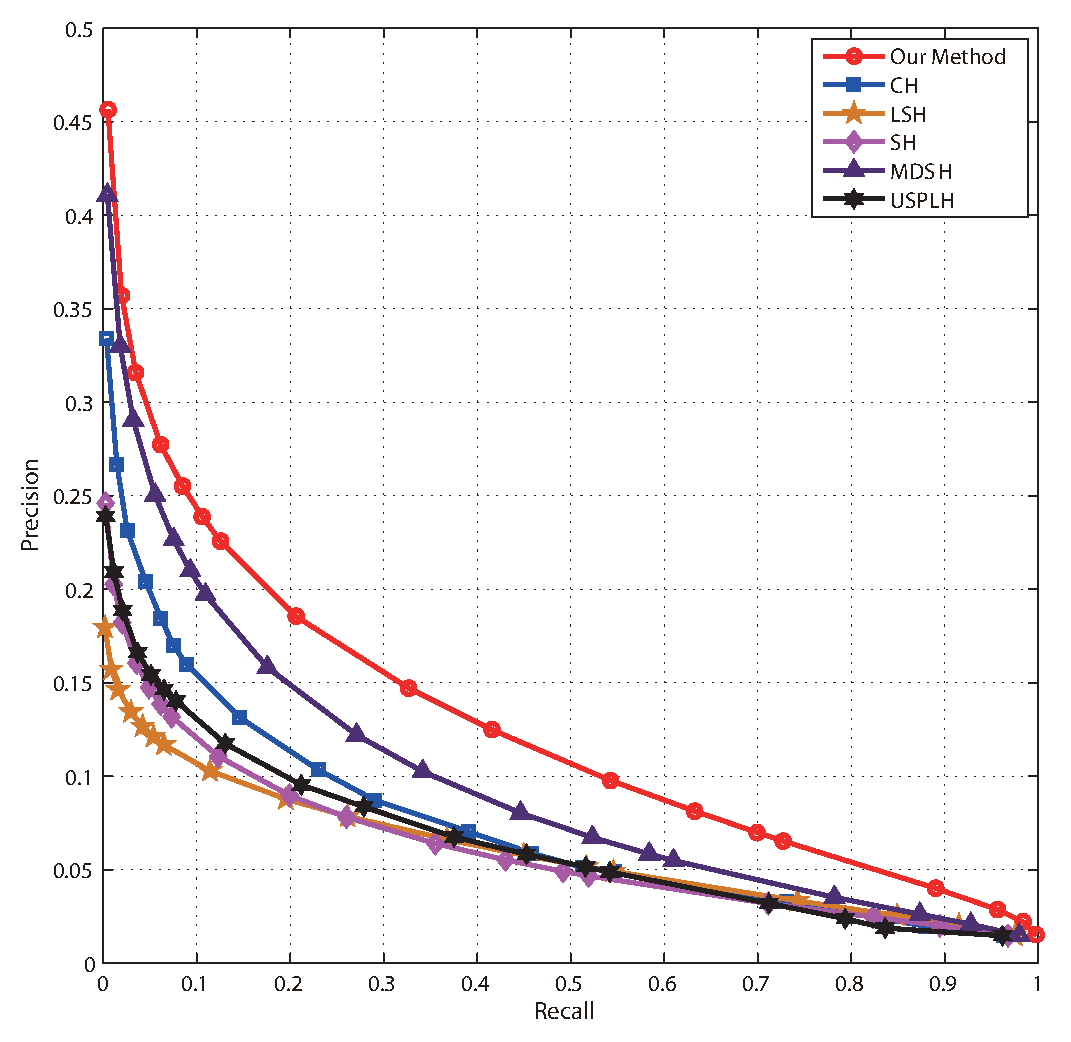
\includegraphics[width= 4.2cm,height = 4.2cm]{images/tiny100k_pr_24bits.eps}}
    \subfigure[\tiny{Precision-Recall curve@32 bits}]{
    \label{figlambda}
    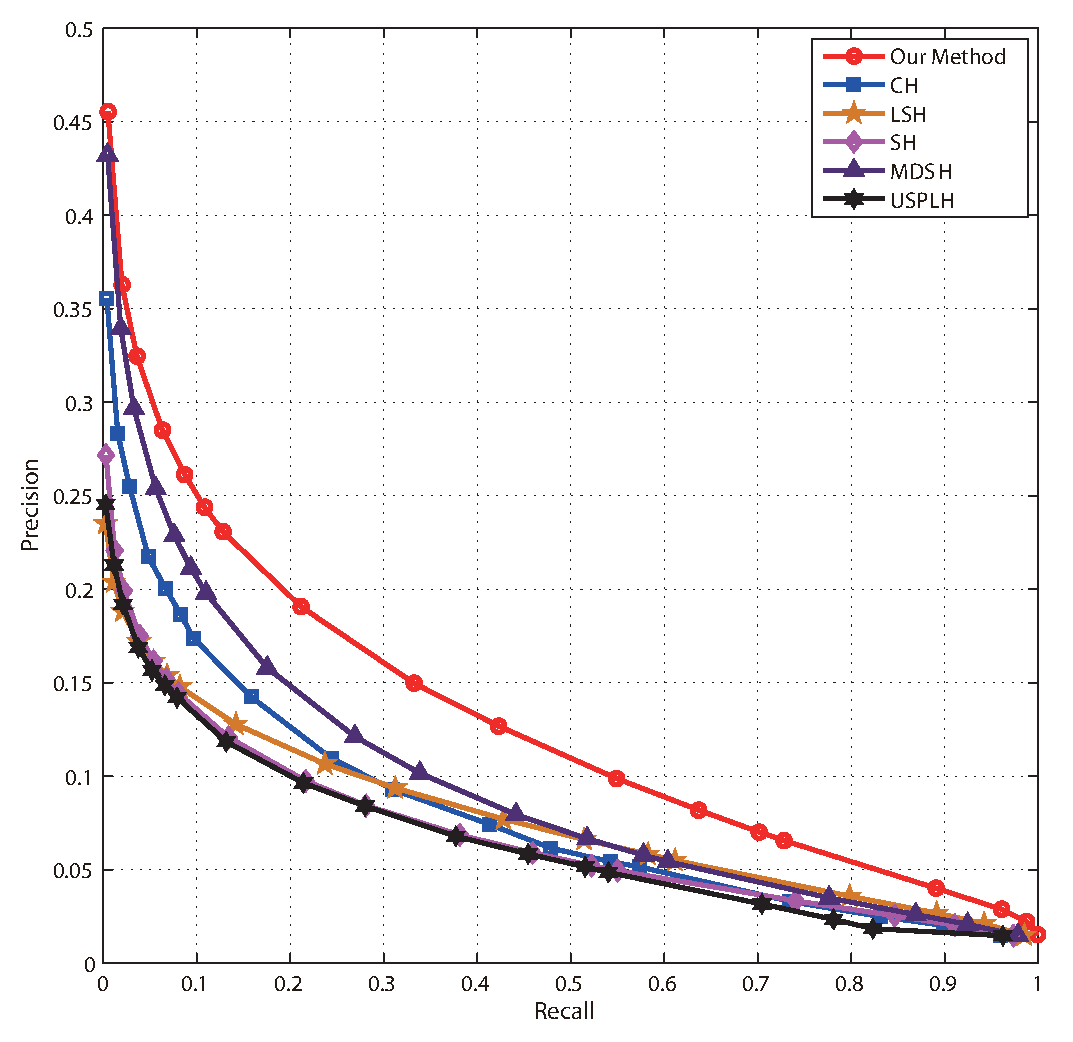
\includegraphics[width= 4.2cm,height = 4.2cm]{images/tiny100k_pr_32bits.eps}}
    \subfigure[\tiny{Precision-Recall curve@48 bits}]{
    \label{figlambda}
    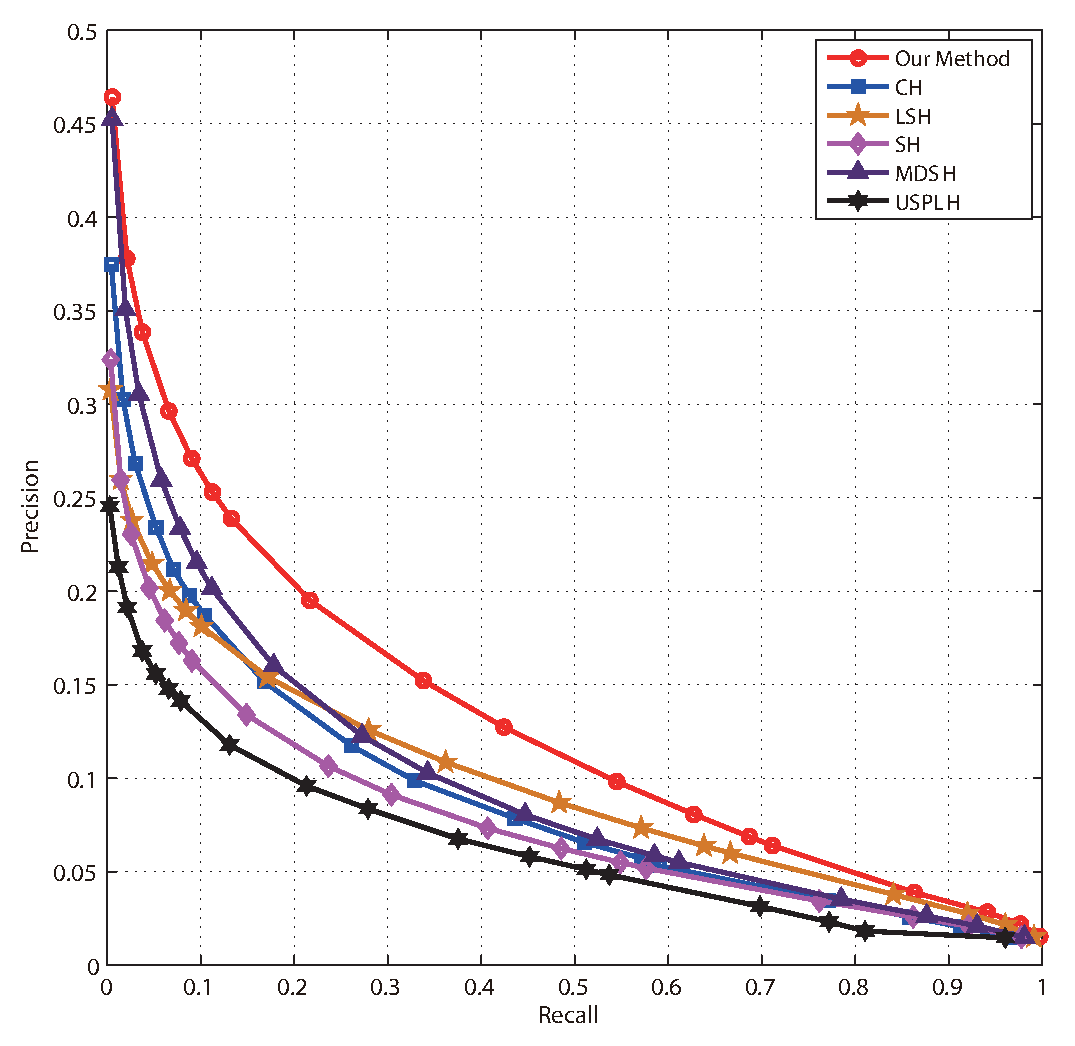
\includegraphics[width= 4.2cm,height = 4.2cm]{images/tiny100k_pr_48bits.eps}}
    \subfigure[\tiny{Recall Curve @16 bits}]{
    \label{figlambda}
    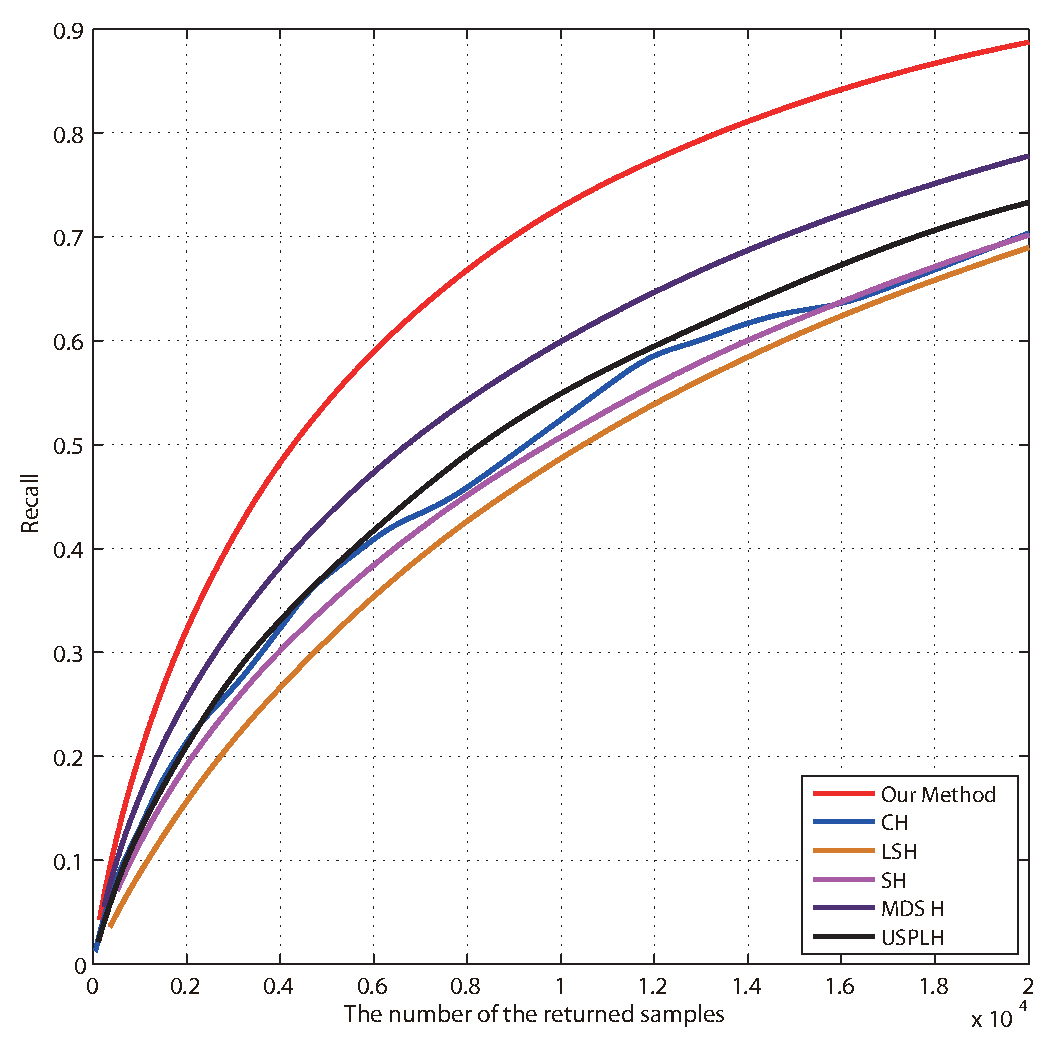
\includegraphics[width= 4.2cm,height = 4.2cm]{images/tiny100k_r_16bits.eps}}
    \subfigure[\tiny{Recall Curve @24 bits}]{
    \label{figsigma}
    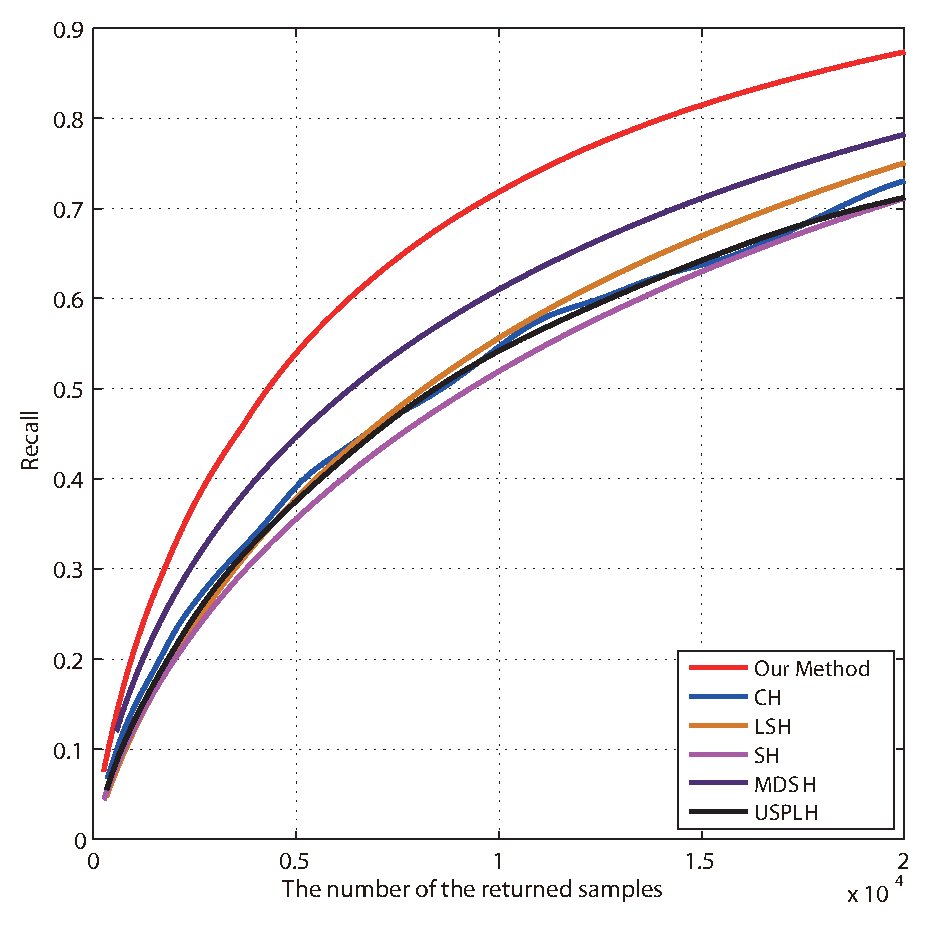
\includegraphics[width= 4.2cm,height = 4.2cm]{images/tiny100k_r_24bits.eps}}
    \subfigure[\tiny{Recall Curve @32 bits}]{
    \label{figlambda}
    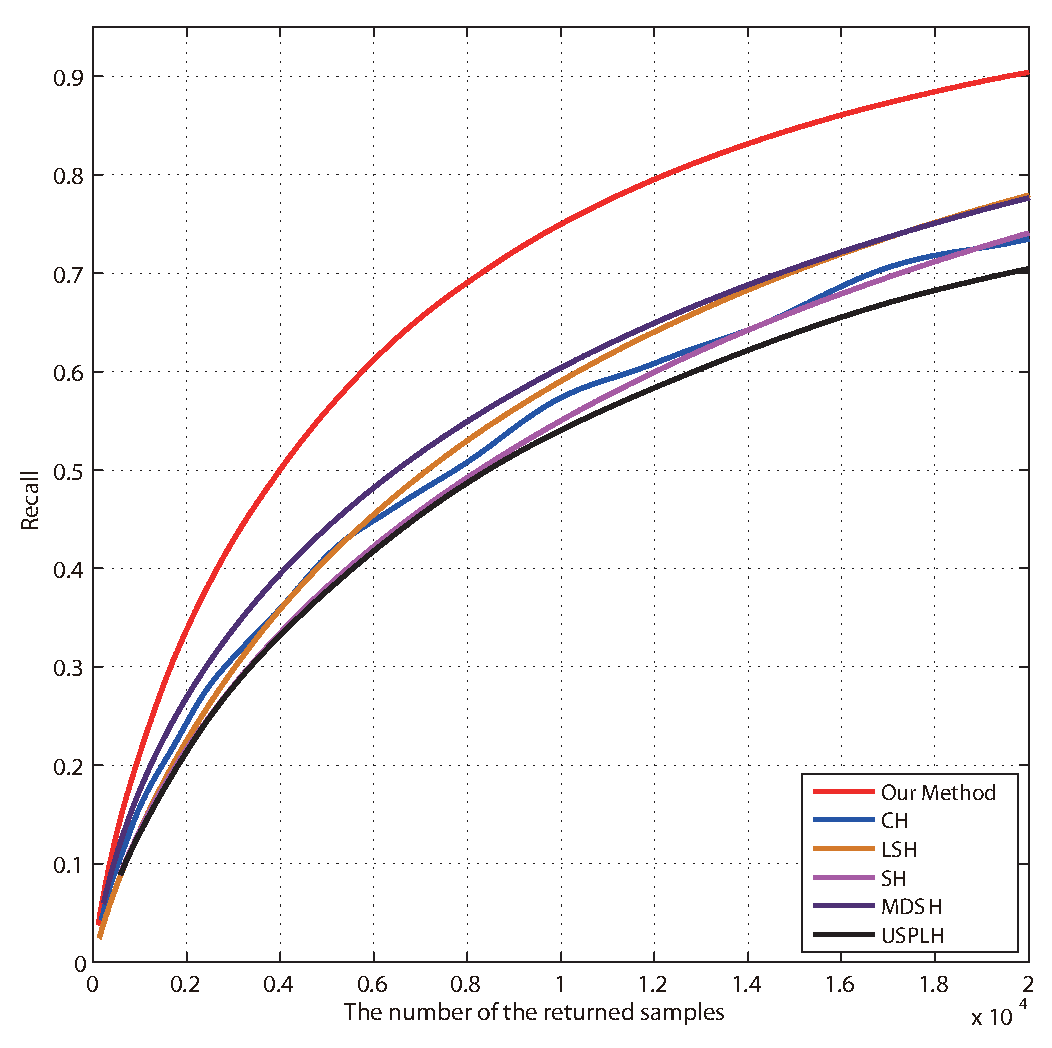
\includegraphics[width= 4.2cm,height = 4.2cm]{images/tiny100k_r_32bits.eps}}
    \subfigure[\tiny{Recall Curve @48 bits}]{
    \label{figlambda}
    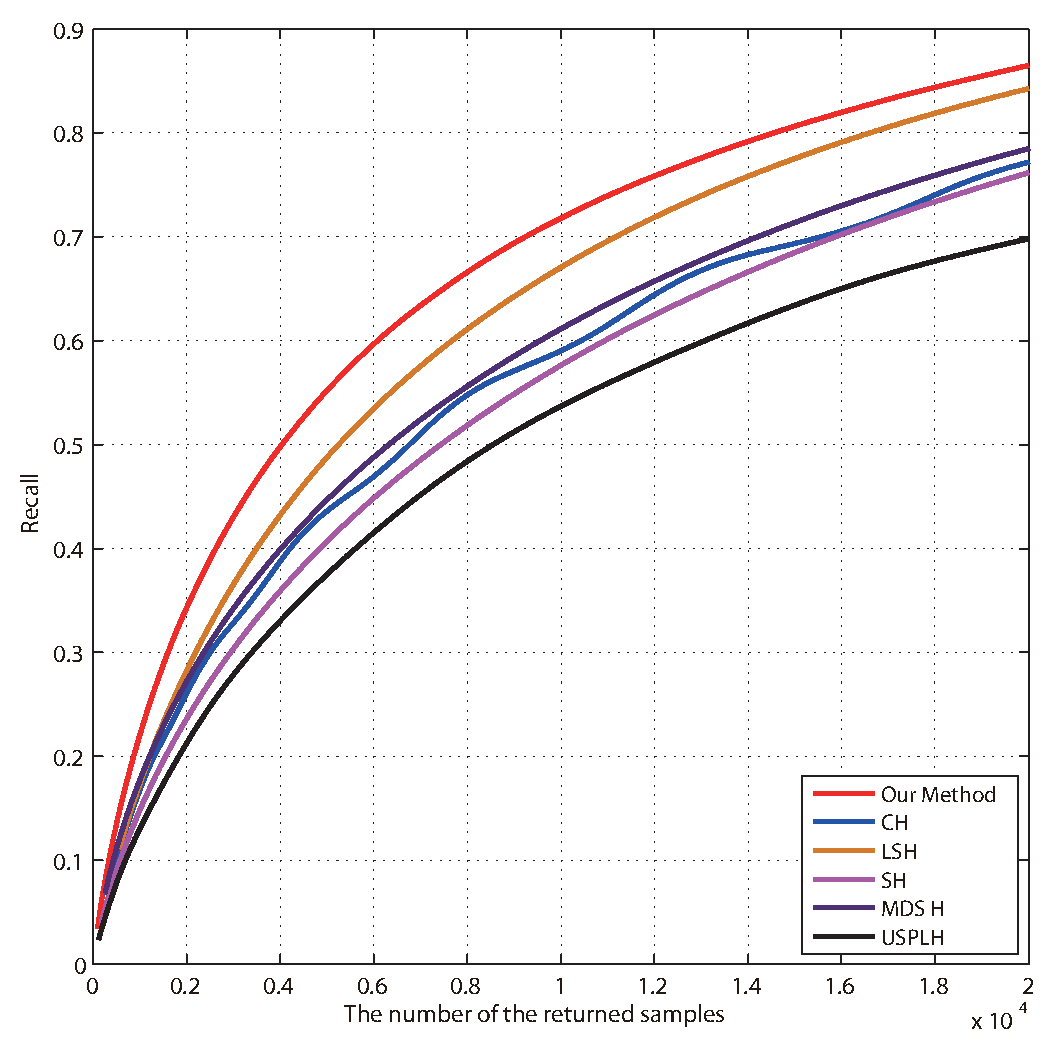
\includegraphics[width= 4.2cm,height = 4.2cm]{images/tiny100k_r_48bits.eps}}
\caption{Precision-Recall curves and Recall-The number of retrieved samples curves of all approaches on 100k Tiny Image dataset.}\label{figtiny100k}
\end{figure*}

\section{Experiments}
%\textbf {Datasets and Experiment setup}
To evaluate the effectiveness of the proposed method, we run large-scale image retrieval on two benchmark datasets, i.e. CIFAR-10 and 100K TinyImage, which have been adopted widely in the evaluation of hashing methods \cite{DBLP:WangKC10-16,DBLP:nipsKulisD09-06,DBLP:cvprLiuWJJC12-07,DBLP:eccvWeissFT12-10,DBLP:cvprGongL11-11}. The first data set CIFAR-10 contains a total of 60K with size $32\times32$ color images from ten class (airplane, automobile, bird, cat, deer, frog, horse, ship and truck). Each class contains 6K samples and the images assigned to a mutually exclusive class label. Every image is represented by a 320-dimensional GIST feature vector. We randomly partitioned it into two parts: a training set of 59K images and a test set of 1K images for query. The second data set is 100K Tiny Images, a subset sampled from the large million Tiny Images. It contains 100K images and each image is presented by a 384-d GIST descriptor. The entire dataset is divided into two parts as well: 90K for training and 10K for test. Since the 100K Tiny Images dataset has no semantic labels, we consider the groundtruth as each test query's $n$ Euclidean nearest neighbors including CIFAR-10. Here $n$ is set to one percent of the size of training data set and the parameters $\alpha$ and $\eta$ in the object function both set to 0.1.
\begin{figure*}[!htb]
\centering
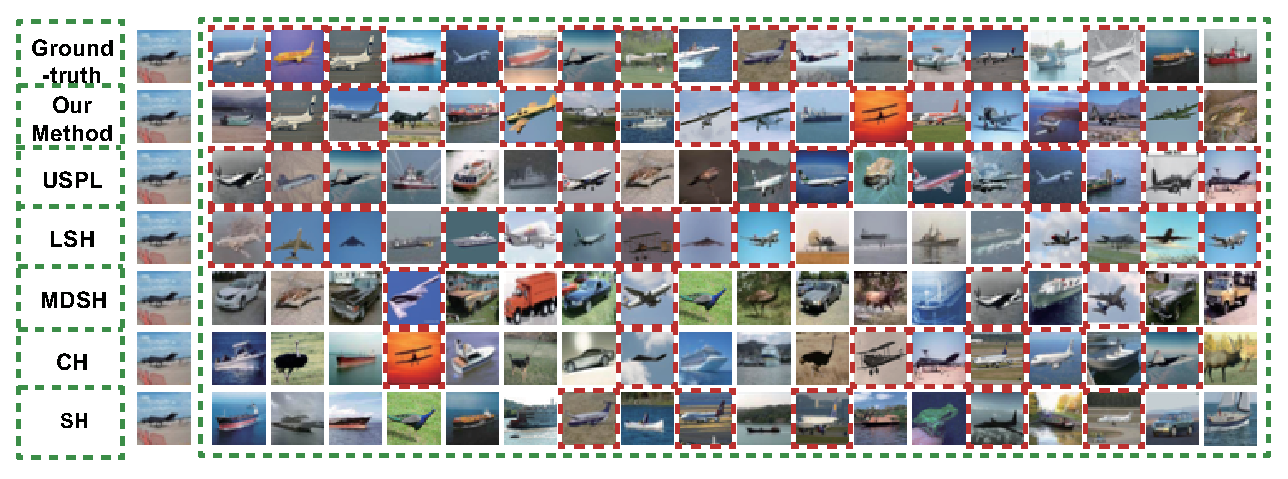
\includegraphics[width=0.83\textwidth]{images/image_rereieve_examples.eps}
\caption{Retrieve an airplane example image using different hash methods}
\label{figexample}
\end{figure*}
%\textbf {Baselines and Evaluation Metrics}

Since the proposed method is based on unsupervised learning, we compare it with five state-of-the-art unsupervised hashing methods including LSH \cite{DBLP:vldbGionisIM99-01}, SH \cite{DBLP:WeissTF08-09}, MDSH \cite{DBLP:eccvWeissFT12-10}, CH \cite{DBLP:iccvXuWLZLY11-12}, and USPLH \cite{DBLP:icmlWangKC10-15}, and \emph{hamming ranking} search strategy is adopted commonly in hashing methods \cite{DBLP:WangKC10-16,DBLP:WeissTF08-09,DBLP:cvprGongL11-11}. \emph{Hamming ranking} sorts all the data points according to their distance to a specific query and the first $N$ samples in the ranked list of the query will be returned. It's an exhaustive linear search method but fast implementation. Besides, it provides better quality measurement of the Hamming embedding though the complexity is linear to the size of the dataset. For a quantitative performance comparison, we adopt precision-recall curses and recall curves of the returned samples number to illustrate the performance of different methods.

The performance comparison on two benchmark datasets are shown in Fig. \ref{figcifar10} and Fig. \ref{figtiny100k}, respectively. From the precision-recall curves in Fig. \ref{figcifar10} and Fig. \ref{figtiny100k}, it clearly observed that the proposed method obtains larger areas under the precision-recall curves compared with the competing hashing methods. It's not very surprising that the proposed hashing method obtains the best performance since the proposed method keeps a sparse structure under $l_{2,1}$-norm constraint while taking adjusted covariance matrix into consideration. Fig. \ref{figcifar10} and Fig. \ref{figtiny100k} also show a little difference on the two benchmark datasets. On CIFAR-10 dataset, the proposed method's advantage is very obvious compared with others methods as the encoding length increases. Meanwhile, On 100K Tiny Images dataset, when the encoding length increases to 48 bits, though the proposed method still performs best, the advantage is no longer obvious. The main reason is that the training set may not be enough while the test query is a little large. Furthermore, the recall curves in Fig. \ref{figcifar10} and Fig. \ref{figtiny100k} also illustrate that the proposed method can obtain higher recall rate for the returned samples number on the two benchmark datasets.

Finally, to obtain a qualitative visual result, Fig. \ref{figexample} shows the retrieved  result of the proposed method and five competing methods on a airplane example image.
\section{Conclusions}
In this paper, a novel sparse reconstruction is proposed by introducing the $l_{2,1}$-norm into SSP framework to preserve potential discrimination information of hash functions. Moreover, we construct an objective function to build a balance between the adjusted covariance matrix and the minimum reconstruction error of data points. The experimental results on two large-scale benchmark datasets show the benefits of our method. In future work, more efficient structure models and labels information will be explored to solve ANN search problem.
\section{Acknowledgments}
This project is supported by the National Basic Research Program of China (973 Program) (Grant No. 2012CB719905), the National Natural Science Foundation of China (Grant Nos: 61125106, 91120302, and 61100079).
%\end{document}  % This is where a 'short' article might terminate

% The following two commands are all you need in the
% initial runs of your .tex file to
% produce the bibliography for the citations in your paper.
%\bibliographystyle{abbrv}
\bibliographystyle{unsrt}
\bibliography{sigproc}  % sigproc.bib is the name of the Bibliography in this case
% You must have a proper ".bib" file
%  and remember to run:
% latex bibtex latex latex
% to resolve all references
%
% ACM needs 'a single self-contained file'!
%
%APPENDICES are optional
%\balancecolumns
\end{document}
